\title{WWW SNT Internal Note}
\author{SNT WWW Team}
\date{\today}

\documentclass[12pt]{article}

%\usepackage[landscape]{geometry}
\usepackage{fullpage}
\usepackage{graphicx}
\usepackage{subfig}
\usepackage{verbatim}
\usepackage{xcolor}

\newcommand{\analysispath}{/home/users/phchang/public_html/analysis/www/code/WWWAnalysisRun2/analysis/plots/WWW2017_v4.0.6/test22}
\newcommand{\fakeratepath}{/home/users/phchang/public_html/analysis/www/code/WWWAnalysisRun2/fakerate/plots/FR2017_v3.0.17/FR2017_analysis_v1.0.0}
\newcommand{\note}[1]{\textbf{\color{red} #1}}

\begin{document}
\maketitle

\begin{abstract}
This contains various tables and plots used for the actual AN of WWW analysis.
\end{abstract}

\section{TODOs}

\begin{itemize}
    \item Lost lepton background estimation
        \begin{itemize}
            \item Lost lepton transfer factor JES needs to be updated.
            \item Lost lepton $m_{SFOS}$ uncertainty of 19.9\% OK?
        \end{itemize}
    \item Non-prompt background estimation
        \begin{itemize}
            \item N.B. Currently, the scale factors are fitted, and the errors on SFs what is varied to obtain the fakerate errors.
        \end{itemize}
    \item VBS $W^{\pm}W^{\pm}$ validation region
        \begin{itemize}
            \item Update the $m_{jj}$ variable to be the same as what was used in 2016 analysis note.
            \item I am not sure if we can say (~22\%) like last time...
            \item $Z\gamma$ sample is missing however...
        \end{itemize}
    \item $t\bar{t}W$ validation region
        \begin{itemize}
            \item Create a similar table done for 2016
        \end{itemize}
    \item $\gamma\rightarrow$ lepton validation region
        \begin{itemize}
            \item \note{Can't do this without $V\gamma$ MC sample! Still not ready AFAIK.}
        \end{itemize}
    \item Charge flip validation region
        \begin{itemize}
            \item Need opposite sign babies. (half a day time for baby production.) But shouldn't be difficult.
            \item Smearing function is probably crucial?
        \end{itemize}
    \item Other random loose ends
        \begin{itemize}
            \item Pre-firing checks for 2017?
        \end{itemize}
    \item Signal region yields
        \begin{itemize}
            \item The plot and table only contains statistical uncertainties.
        \end{itemize}
    \item Statistical interpretation
        \begin{itemize}
            \item Some of it comes from 2016. Still needs some updates.
            \item Several systematics table needs to be updated properly.
        \end{itemize}
\end{itemize}


\section{Lost Lepton Control Region}

\input{\analysispath/lostlep_cr_yield}

\begin{figure}[!htb]
    \centering
    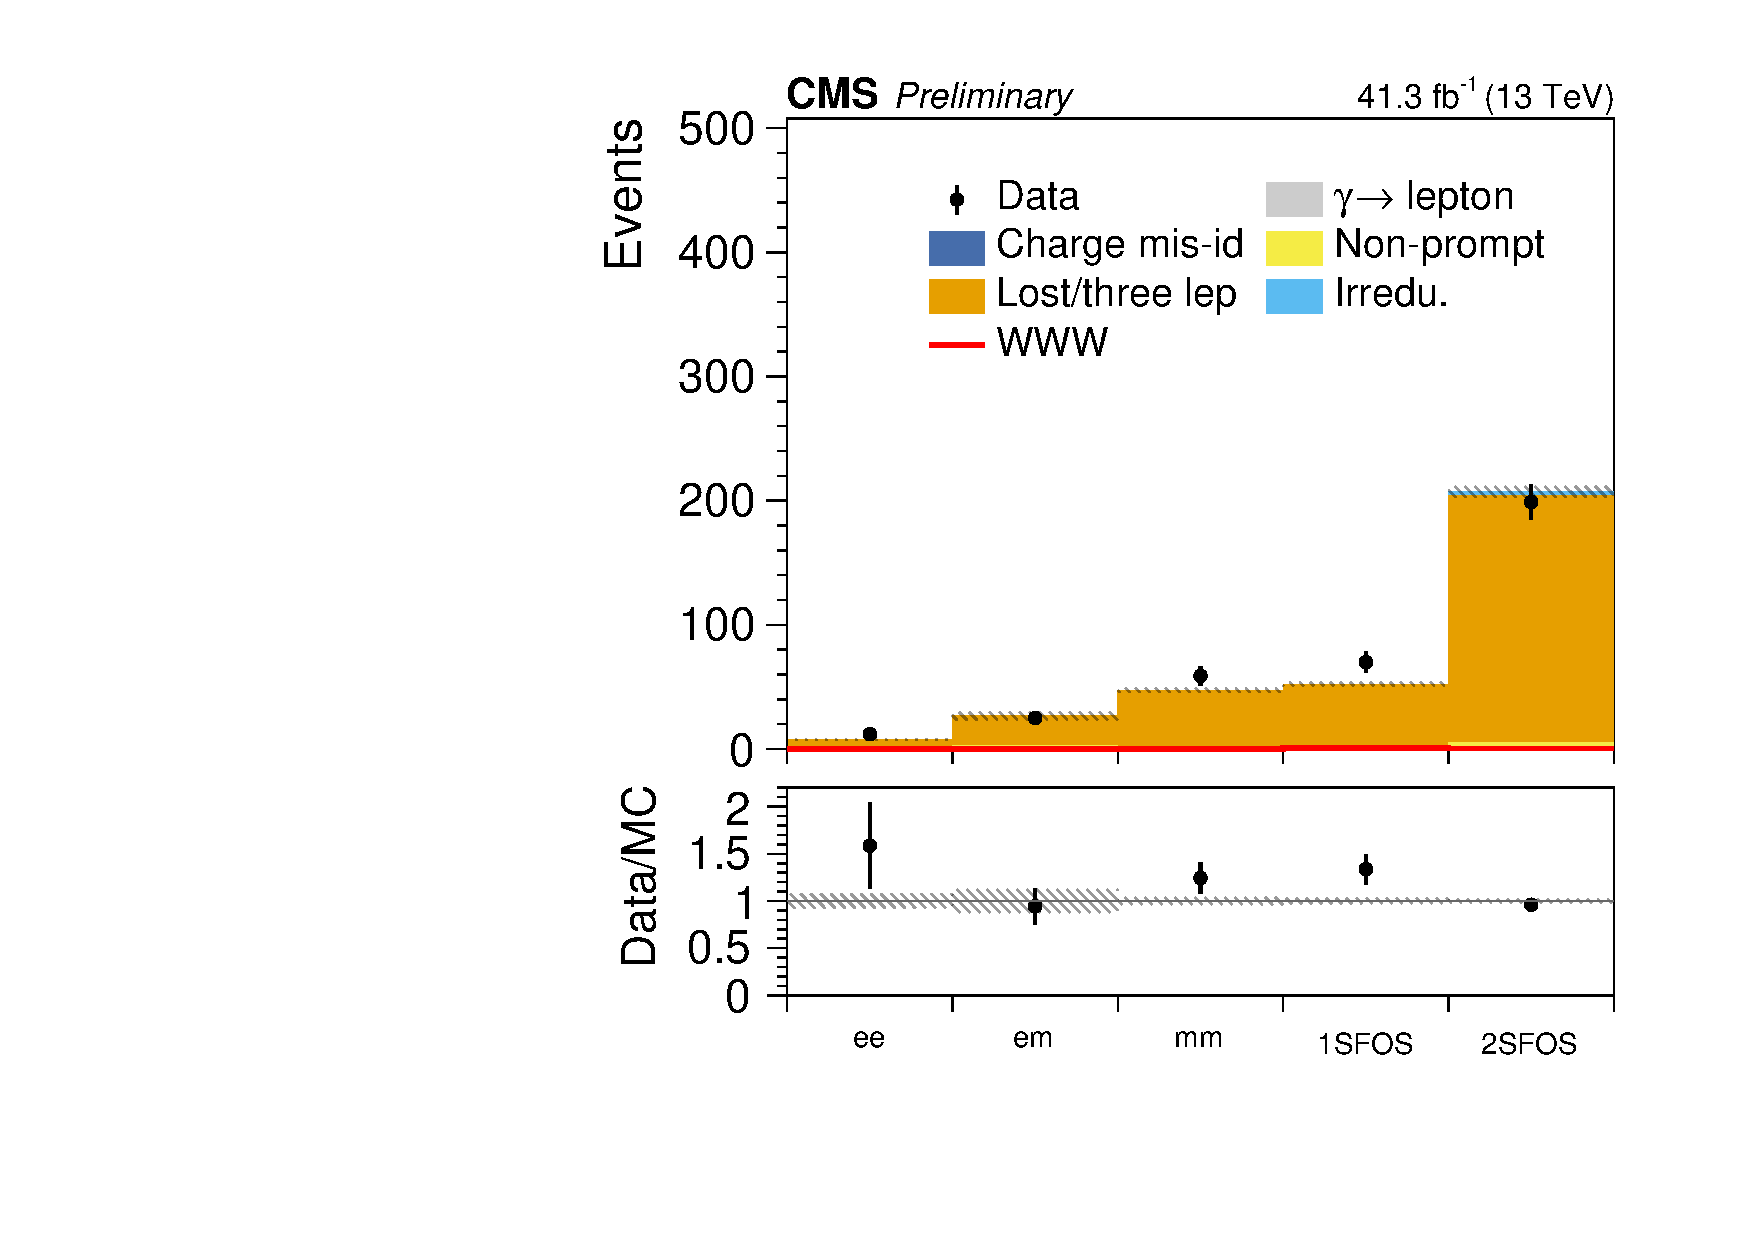
\includegraphics[width=0.80\textwidth]{\analysispath/lostlep_cr_yield.pdf}
    \caption{
        \label{fig:2017:lostlepcr} Lost lepton control region for 2017 data.
    }
\end{figure}


\input{\analysispath/lostlep_exp_syst}

\begin{figure}[!htb]
    \centering
    \subfloat[][]{\includegraphics[width=0.45\textwidth]{\analysispath/lostlep_cr_ss_msfos.pdf}\label{fig:2017:lostlepcr:msfos:ss}}
    \subfloat[][]{\includegraphics[width=0.45\textwidth]{\analysispath/lostlep_cr_3l_msfos.pdf}\label{fig:2017:lostlepcr:msfos:3l}}\\
    \subfloat[][]{\includegraphics[width=0.45\textwidth]{\analysispath/lostlep_cr_ss_mjj.pdf}\label{fig:2017:lostlepcr:mjj:ss}}
    \caption{
        \label{fig:2017:lostlepcr:modeling} Lost lepton control region, efficiencies and extrapolation checks
        \subref{fig:2017:lostlepcr:msfos:ss}{ The $m_{SFOS}$ distribution in lost lepton control regions for same-sign channels.} 
        \subref{fig:2017:lostlepcr:msfos:3l}{ The $m_{SFOS}$ distribution in lost lepton control regions for three-lepton channels.} 
        \subref{fig:2017:lostlepcr:mjj:ss}{ The $m_{jj}$ distribution in lost lepton control regions for same-sign channels.} 
    }
\end{figure}

\input{\analysispath/lostlep_eff_msfos_ss}
\input{\analysispath/lostlep_ratio_msfos_3l}
\input{\analysispath/lostlep_eff_mjj_ss}

\clearpage

\section{Non-prompt backgrounds}

\begin{figure}[!htb]
    \centering
    \subfloat[][]{\includegraphics[width=0.45\textwidth]{\fakeratepath/ss/plot/OneElEWKCR__Nvtx.pdf}\label{fig:2017:fake:nvtx:ss:el}}
    \subfloat[][]{\includegraphics[width=0.45\textwidth]{\fakeratepath/ss/plot/OneMuEWKCR__Nvtx.pdf}\label{fig:2017:fake:nvtx:ss:mu}}\\
    \subfloat[][]{\includegraphics[width=0.45\textwidth]{\fakeratepath/3l/plot/OneElEWKCR__Nvtx.pdf}\label{fig:2017:fake:nvtx:3l:el}}
    \subfloat[][]{\includegraphics[width=0.45\textwidth]{\fakeratepath/3l/plot/OneMuEWKCR__Nvtx.pdf}\label{fig:2017:fake:nvtx:3l:mu}}
    \caption{
        \label{fig:2017:fake:nvtx} Checking number of vertex distribution after applying prescales.
        \subref{fig:2017:fake:nvtx:ss:el}{ The number of vertex distribution in one lepton control region for same-sign electron ID.} 
        \subref{fig:2017:fake:nvtx:ss:mu}{ The number of vertex distribution in one lepton control region for same-sign muon ID.} 
        \subref{fig:2017:fake:nvtx:3l:el}{ The number of vertex distribution in one lepton control region for three-lepton electron ID.} 
        \subref{fig:2017:fake:nvtx:3l:mu}{ The number of vertex distribution in one lepton control region for three-lepton muon ID.} 
    }
\end{figure}

\begin{figure}[!htb]
    \centering
    \subfloat[][]{\includegraphics[width=0.45\textwidth]{\fakeratepath/ss/plot/TwoElHLT23__Mll.pdf}\label{fig:2017:fake:prescale:ss:el}}
    \subfloat[][]{\includegraphics[width=0.45\textwidth]{\fakeratepath/ss/plot/TwoMuHLT17__Mll.pdf}\label{fig:2017:fake:prescale:ss:mu}}\\
    \subfloat[][]{\includegraphics[width=0.45\textwidth]{\fakeratepath/3l/plot/TwoElHLT23__Mll.pdf}\label{fig:2017:fake:prescale:3l:el}}
    \subfloat[][]{\includegraphics[width=0.45\textwidth]{\fakeratepath/3l/plot/TwoMuHLT17__Mll.pdf}\label{fig:2017:fake:prescale:3l:mu}}
    \caption{
        \label{fig:2017:fake:prescale} Even after applying prescale, some residual difference is corrected by obtaining a scale factor by comparing the expected MC yields to Z boson events from data.
        \subref{fig:2017:fake:prescale:ss:el}{ The $m_{ll}$ distribution in two leptons control region with same-sign electron ID.} 
        \subref{fig:2017:fake:prescale:ss:mu}{ The $m_{ll}$ distribution in two leptons control region with same-sign muon ID.} 
        \subref{fig:2017:fake:prescale:3l:el}{ The $m_{ll}$ distribution in two leptons control region with three-lepton electron ID.} 
        \subref{fig:2017:fake:prescale:3l:mu}{ The $m_{ll}$ distribution in two leptons control region with three-lepton muon ID.} 
    }
\end{figure}

\begin{figure}[!htb]
    \centering
    \subfloat[][]{\includegraphics[width=0.45\textwidth]{\fakeratepath/ss/plot/OneElHighMET__MT.pdf}\label{fig:2017:fake:mt:ss:el}}
    \subfloat[][]{\includegraphics[width=0.45\textwidth]{\fakeratepath/ss/plot/OneMuHighMET__MT.pdf}\label{fig:2017:fake:mt:ss:mu}}\\
    \subfloat[][]{\includegraphics[width=0.45\textwidth]{\fakeratepath/3l/plot/OneElHighMET__MT.pdf}\label{fig:2017:fake:mt:3l:el}}
    \subfloat[][]{\includegraphics[width=0.45\textwidth]{\fakeratepath/3l/plot/OneMuHighMET__MT.pdf}\label{fig:2017:fake:mt:3l:mu}}
    \caption{
        \label{fig:2017:fake:mt} The $m_{T}$ distribution in high MET region where the window of 80 GeV $< m_{T} <$ 120 GeV is used as a control region to obtain scale factors to apply to the prompt lepton contribution in the measurement region where the fake rate is derived.
        \subref{fig:2017:fake:mt:ss:el}{ The $m_{T}$ distribution in one lepton control region for same-sign electron ID.} 
        \subref{fig:2017:fake:mt:ss:mu}{ The $m_{T}$ distribution in one lepton control region for same-sign muon ID.} 
        \subref{fig:2017:fake:mt:3l:el}{ The $m_{T}$ distribution in one lepton control region for three-lepton electron ID.} 
        \subref{fig:2017:fake:mt:3l:mu}{ The $m_{T}$ distribution in one lepton control region for three-lepton muon ID.} 
    }
\end{figure}

\begin{figure}[!htb]
    \centering
    \subfloat[][]{\includegraphics[width=0.45\textwidth]{\fakeratepath/ss/plot/OneElTightMR__ptcorrvarbin.pdf}\label{fig:2017:fake:ptcorrvarbin:ss:el}}
    \subfloat[][]{\includegraphics[width=0.45\textwidth]{\fakeratepath/ss/plot/OneMuTightMR__ptcorrvarbin.pdf}\label{fig:2017:fake:ptcorrvarbin:ss:mu}}\\
    \subfloat[][]{\includegraphics[width=0.45\textwidth]{\fakeratepath/3l/plot/OneElTightMR__ptcorrvarbin.pdf}\label{fig:2017:fake:ptcorrvarbin:3l:el}}
    \subfloat[][]{\includegraphics[width=0.45\textwidth]{\fakeratepath/3l/plot/OneMuTightMR__ptcorrvarbin.pdf}\label{fig:2017:fake:ptcorrvarbin:3l:mu}}
    \caption{
        \label{fig:2017:fake:ptcorrvarbin} The $p_{T,corr}$ distribution in measurement region with one tight lepton.
        \subref{fig:2017:fake:ptcorrvarbin:ss:el}{ The $p_{T,corr}$ one lepton tight measurement region for same-sign electron ID.} 
        \subref{fig:2017:fake:ptcorrvarbin:ss:mu}{ The $p_{T,corr}$ one lepton tight measurement region for same-sign muon ID.} 
        \subref{fig:2017:fake:ptcorrvarbin:3l:el}{ The $p_{T,corr}$ one lepton tight measurement region for three-lepton electron ID.} 
        \subref{fig:2017:fake:ptcorrvarbin:3l:mu}{ The $p_{T,corr}$ one lepton tight measurement region for three-lepton muon ID.} 
    }
\end{figure}

\begin{figure}[!htb]
    \centering
    \subfloat[][]{\includegraphics[width=0.45\textwidth]{\fakeratepath/ss/plot/OneElMR__ptcorrvarbin.pdf}\label{fig:2017:fake:loose:ptcorrvarbin:ss:el}}
    \subfloat[][]{\includegraphics[width=0.45\textwidth]{\fakeratepath/ss/plot/OneMuMR__ptcorrvarbin.pdf}\label{fig:2017:fake:loose:ptcorrvarbin:ss:mu}}\\
    \subfloat[][]{\includegraphics[width=0.45\textwidth]{\fakeratepath/3l/plot/OneElMR__ptcorrvarbin.pdf}\label{fig:2017:fake:loose:ptcorrvarbin:3l:el}}
    \subfloat[][]{\includegraphics[width=0.45\textwidth]{\fakeratepath/3l/plot/OneMuMR__ptcorrvarbin.pdf}\label{fig:2017:fake:loose:ptcorrvarbin:3l:mu}}
    \caption{
        \label{fig:2017:fake:loose:ptcorrvarbin} The $p_{T,corr}$ distribution in measurement region with one loose lepton.
        \subref{fig:2017:fake:loose:ptcorrvarbin:ss:el}{ The $p_{T,corr}$ one lepton loose measurement region for same-sign electron ID.} 
        \subref{fig:2017:fake:loose:ptcorrvarbin:ss:mu}{ The $p_{T,corr}$ one lepton loose measurement region for same-sign muon ID.} 
        \subref{fig:2017:fake:loose:ptcorrvarbin:3l:el}{ The $p_{T,corr}$ one lepton loose measurement region for three-lepton electron ID.} 
        \subref{fig:2017:fake:loose:ptcorrvarbin:3l:mu}{ The $p_{T,corr}$ one lepton loose measurement region for three-lepton muon ID.} 
    }
\end{figure}

\begin{figure}[!htb]
    \centering
    \subfloat[][]{\includegraphics[width=0.45\textwidth]{\fakeratepath/ss/fakerate/OneElTightMR__ptcorrvarbin__OneElMR__ptcorrvarbin.pdf}\label{fig:2017:fake:fakerate:ptcorrvarbin:ss:el}}
    \subfloat[][]{\includegraphics[width=0.45\textwidth]{\fakeratepath/ss/fakerate/OneMuTightMR__ptcorrvarbin__OneMuMR__ptcorrvarbin.pdf}\label{fig:2017:fake:fakerate:ptcorrvarbin:ss:mu}}\\
    \subfloat[][]{\includegraphics[width=0.45\textwidth]{\fakeratepath/3l/fakerate/OneElTightMR__ptcorrvarbin__OneElMR__ptcorrvarbin.pdf}\label{fig:2017:fake:fakerate:ptcorrvarbin:3l:el}}
    \subfloat[][]{\includegraphics[width=0.45\textwidth]{\fakeratepath/3l/fakerate/OneMuTightMR__ptcorrvarbin__OneMuMR__ptcorrvarbin.pdf}\label{fig:2017:fake:fakerate:ptcorrvarbin:3l:mu}}
    \caption{
        \label{fig:2017:fake:fakerate:ptcorrvarbin} Fake rate measured as a function of $p_{T,corr}$.
        \subref{fig:2017:fake:fakerate:ptcorrvarbin:ss:el}{ The fake rate for same-sign electron ID.}
        \subref{fig:2017:fake:fakerate:ptcorrvarbin:ss:mu}{ The fake rate for same-sign muon ID.}
        \subref{fig:2017:fake:fakerate:ptcorrvarbin:3l:el}{ The fake rate for three-lepton electron ID.}
        \subref{fig:2017:fake:fakerate:ptcorrvarbin:3l:mu}{ The fake rate for three-lepton muon ID.}
    }
\end{figure}

\begin{figure}[!htb]
    \centering
    \subfloat[][]{\includegraphics[width=0.45\textwidth]{\fakeratepath/ss/fakerate/OneElTightMR__ptcorretarolledcoarse__OneElMR__ptcorretarolledcoarse.pdf}\label{fig:2017:fake:fakerate2d:ptcorretarolledcoarse:ss:el}}
    \subfloat[][]{\includegraphics[width=0.45\textwidth]{\fakeratepath/ss/fakerate/OneMuTightMR__ptcorretarolledcoarse__OneMuMR__ptcorretarolledcoarse.pdf}\label{fig:2017:fake:fakerate2d:ptcorretarolledcoarse:ss:mu}}\\
    \subfloat[][]{\includegraphics[width=0.45\textwidth]{\fakeratepath/3l/fakerate/OneElTightMR__ptcorretarolledcoarse__OneElMR__ptcorretarolledcoarse.pdf}\label{fig:2017:fake:fakerate2d:ptcorretarolledcoarse:3l:el}}
    \subfloat[][]{\includegraphics[width=0.45\textwidth]{\fakeratepath/3l/fakerate/OneMuTightMR__ptcorretarolledcoarse__OneMuMR__ptcorretarolledcoarse.pdf}\label{fig:2017:fake:fakerate2d:ptcorretarolledcoarse:3l:mu}}
    \caption{
        \label{fig:2017:fake:fakerate2d:ptcorretarolledcoarse} Fake rate measured as a function of $p_{T,corr}$ and $|\eta|$. Each bin is labeled by its phase-space. The first pair of numbers indicate the $p_{T,corr}$ phase space boundaries, and the second pair of numbers indicate the $|\eta|$ phase space boundaries.
        \subref{fig:2017:fake:fakerate2d:ptcorretarolledcoarse:ss:el}{ The fake rate for same-sign electron ID.}
        \subref{fig:2017:fake:fakerate2d:ptcorretarolledcoarse:ss:mu}{ The fake rate for same-sign muon ID.}
        \subref{fig:2017:fake:fakerate2d:ptcorretarolledcoarse:3l:el}{ The fake rate for three-lepton electron ID.}
        \subref{fig:2017:fake:fakerate2d:ptcorretarolledcoarse:3l:mu}{ The fake rate for three-lepton muon ID.}
    }
\end{figure}


\input{\fakeratepath/ss/scalefactors}
\input{\fakeratepath/3l/scalefactors}

\section{VBS Validation Region}

\begin{figure}[!htb]
    \centering
    \subfloat[][]{\includegraphics[width=0.45\textwidth]{\analysispath/vbsww_cr_ss_mjj.pdf}\label{fig:2017:vbswwcr:ss:mjj}}
    \subfloat[][]{\includegraphics[width=0.45\textwidth]{\analysispath/vbsww_cr_ss_detajj.pdf}\label{fig:2017:vbswwcr:ss:detajj}}
    \caption{
        \label{fig:2017:vbswwcr:ss} VBS $W^{\pm}W^{\pm}$ control region plots.
        \subref{fig:2017:vbswwcr:ss:mjj}{ \note{This isn't the same variable as 2016 analysis note.} The invariant mass of the two leading jets across all $\eta$ region. }
        \subref{fig:2017:vbswwcr:ss:detajj}{ The $\Delta_{jj}$ of two leading jets within central regions. }
    }
\end{figure}

\clearpage

\section{$t\bar{t}W$ Validation Region}

\begin{figure}[!htb]
    \centering
    \includegraphics[width=0.45\textwidth]{\analysispath/ttw_cr_ss_nb.pdf}\label{fig:2017:ttwcr:ss:nb}
    \caption{
        \label{fig:2017:ttwcr:ss} The $n_{b}$ distribution in $t\bar{t}W$ validation region.
    }
\end{figure}

\clearpage

\section{Signal Region Yields}

\begin{figure}[!htb]
    \centering
    \includegraphics[width=0.80\textwidth]{\analysispath/sr_yield.pdf}\label{fig:2017:sr}
    \caption{
        \label{fig:2017:sr} Signal region yields after applying background estimation methods. The uncertainty band only includes statistical uncertainties.
    }
\end{figure}

\input{\analysispath/sr_yield}

\clearpage

\section{Statistical interpretation}

\subsection{$m_{jj}$-in ee}
\scalebox{0.4}{\parbox{2.0\textwidth}{\verbatiminput{\analysispath/datacard_SRSSee.txt}}}
\subsection{$m_{jj}$-in em}
\scalebox{0.4}{\parbox{2.0\textwidth}{\verbatiminput{\analysispath/datacard_SRSSem.txt}}}
\subsection{$m_{jj}$-in mm}
\scalebox{0.4}{\parbox{2.0\textwidth}{\verbatiminput{\analysispath/datacard_SRSSmm.txt}}}
\subsection{$m_{jj}$-out ee}
\scalebox{0.4}{\parbox{2.0\textwidth}{\verbatiminput{\analysispath/datacard_SRSSSideee.txt}}}
\subsection{$m_{jj}$-out em}
\scalebox{0.4}{\parbox{2.0\textwidth}{\verbatiminput{\analysispath/datacard_SRSSSideem.txt}}}
\subsection{$m_{jj}$-out mm}
\scalebox{0.4}{\parbox{2.0\textwidth}{\verbatiminput{\analysispath/datacard_SRSSSidemm.txt}}}
\subsection{0SFOS}
\scalebox{0.4}{\parbox{2.0\textwidth}{\verbatiminput{\analysispath/datacard_SR0SFOS.txt}}}
\subsection{1SFOS}
\scalebox{0.4}{\parbox{2.0\textwidth}{\verbatiminput{\analysispath/datacard_SR1SFOS.txt}}}
\subsection{2SFOS}
\scalebox{0.4}{\parbox{2.0\textwidth}{\verbatiminput{\analysispath/datacard_SR2SFOS.txt}}}



\end{document}
